%%%%%%%%%%%%%%%%%%%%%%%%%%%%%%%%%%%%%%START PREAMBLE 
\documentclass{article}

%Required: You must have these
\usepackage{Sweave}
\usepackage{graphicx}
\usepackage{tabularx}
\usepackage{hyperref}
\usepackage{natbib}
\usepackage{pdflscape}
\usepackage{array}
\usepackage{gensymb}
%\usepackage[backend=bibtex]{biblatex}
%Strongly recommended
  %put your figures in one place
%\SweaveOpts{prefix.string=figures/, eps=FALSE} 
%you'll want these for pretty captioning
\usepackage[small]{caption}

\setkeys{Gin}{width=0.8\textwidth}  %make the figs 50 perc textwidth
\setlength{\captionmargin}{30pt}
\setlength{\abovecaptionskip}{10pt}
\setlength{\belowcaptionskip}{10pt}
%change margins
 \topmargin -1.5cm        
 \oddsidemargin -0.04cm   
 \evensidemargin -0.04cm  % same as oddside margin but for left-hand pages
 \textwidth 16.59cm
 \textheight 21.94cm 
 %\pagestyle{empty}       % Uncomment if don't want page numbers
 \parskip 7.2pt           % sets spacing between paragraphs
 %\renewcommand{\baselinestretch}{1.5} 	% Uncomment for 1.5 spacing between lines
\parindent 0pt% sets leading space for paragraphs
\usepackage{setspace}
%\doublespacing

%For fancy headers
%\usepackage{fancyhdr}
%\pagestyle{fancy}
%\fancyhead[LO]{}
%\fancyhead[RO]{2019}
 
%%%%%%%%%%%%%%%%%%%%%%%%%%%%%%%%%%%%%%END PREAMBLE THAT IS THE SAME FOR ALL EXAMPLES

%Start of the document
\begin{document}

%\SweaveOpts{concordance=TRUE}
 \bibliographystyle{..//refs/bibstyles/amnat.bst}
\title{How much is enough and where to start? Quantifying and prioritizing locations for reductions in urbanization effects to benefit coho salmon populations} % perspective paper for OSPREE analyses

\author{A.K. Ettinger, E. Buhle, B. Feist, J. N. Scholz, J. Spromberg, P. Levin}
%\date{\today}
\maketitle  %put the fancy title on
%\tableofcontents      %add a table of contents
%\clearpage
%goal is NCC Perspective
%Need to submit "brief synopsis through our online submission system before preparing a manuscript for formal submission. The synopsis should outline the topics that will be covered, list any recent, key publications in the area, and state the last time the topic was reviewed (if it has been reviewed previously)."
%should be presented using simple prose, avoiding excessive jargon and technical detail.
%3,000–5,000 words and typically include 4–6 display items (figures, tables or boxes). 
%up to 100 references; citations should be selective. 
%%%%%%%%%%%%%%%%%%%%%%%%%%%%%%%%%%%%%%%%%%%%%%%%%%%

\section*{Title Ideas}
\begin{itemize}
\item How much is enough and where to start? Quantifying and prioritizing locations for reductions in urbanization effects to benefit coho salmon populations
\item How much is enough and where to start? Quantifying and prioritizing locations for conservation action with limited biological data
\item How much is enough and where to start? Applying structural equation models and Bayesian multilevel models to conservation prioritization
\item How much is enough and where to start? Applying models of mortality rates in threatened coho populations to prioritize conservation actions
\end{itemize}
\section*{Introduction}
\section*{Methods}
\section*{Results}
\section*{Discussion}
\section*{Conclusion}
\bibliography{..//..//fishphen/refs/noaalib.bib}
\section*{Acknowledgements}
\section* {Figures}

%\begin{figure}[h!]
%\centering
%\noindent \includegraphics[width=0.75\textwidth]{..//analysis/results/figures/framework.pdf}
%\caption{\textbf{Framework for prioritizing areas of conseration and restoration action} using %site-level estimates of coho pre-spawn mortality and urbanization effects.}
%\label{fig:frame}
%\end{figure}

\begin{figure}[h!]
\centering
\noindent 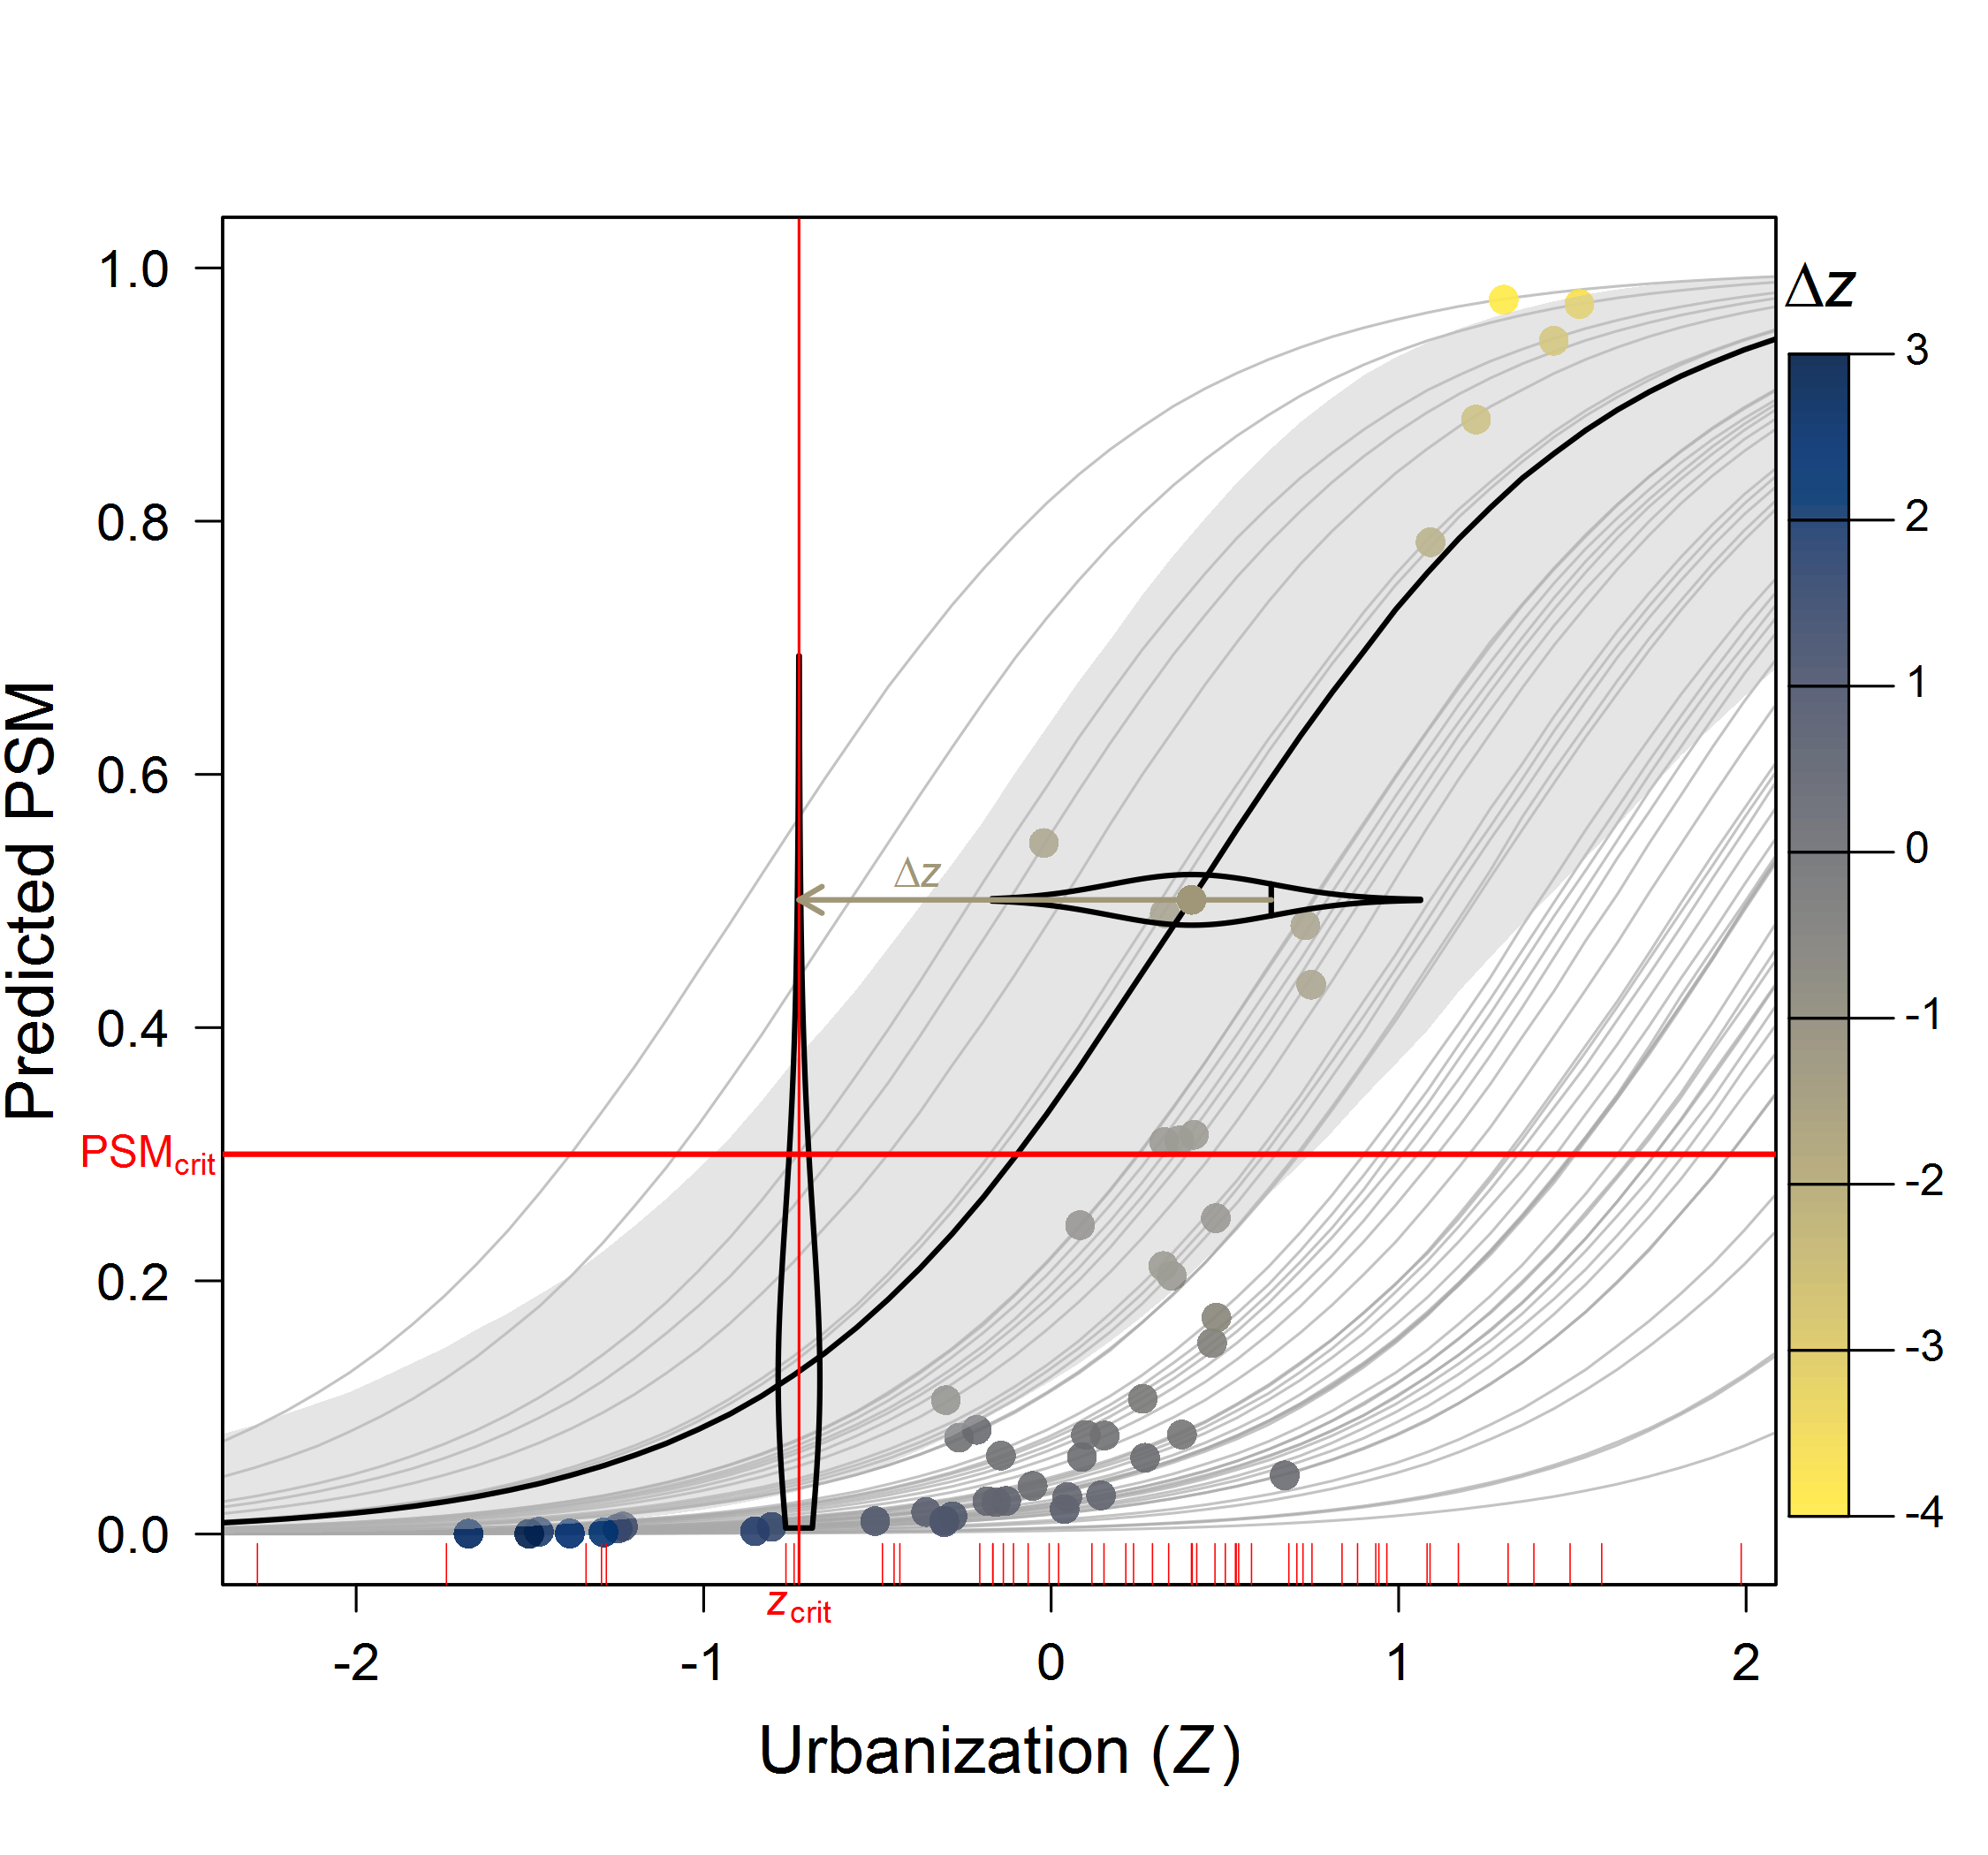
\includegraphics[width=0.75\textwidth]{..//analysis/results/figures/psm_z_threshold.png}
\caption{\textbf{Relationship between estimated pre-spawn mortality and urbanization} based on the structural equation and multi-level modeling in \citep{feist2017}.}
\label{fig:psmz}
\end{figure}

%%%%%%%%%%%%%%%%%%%%%%%%%%%%%%%%%%%%%%%%
\end{document}
%%%%%%%%%%%%%%%%%%%%%%%%%%%%%%%%%%%%%%%%
